\documentclass{standalone}

\usepackage{tikz}
\usepackage{varwidth}

\usetikzlibrary{matrix}
\usetikzlibrary{automata,arrows,calc,positioning}
\usetikzlibrary{shapes.geometric}

\begin{document}

\par\noindent

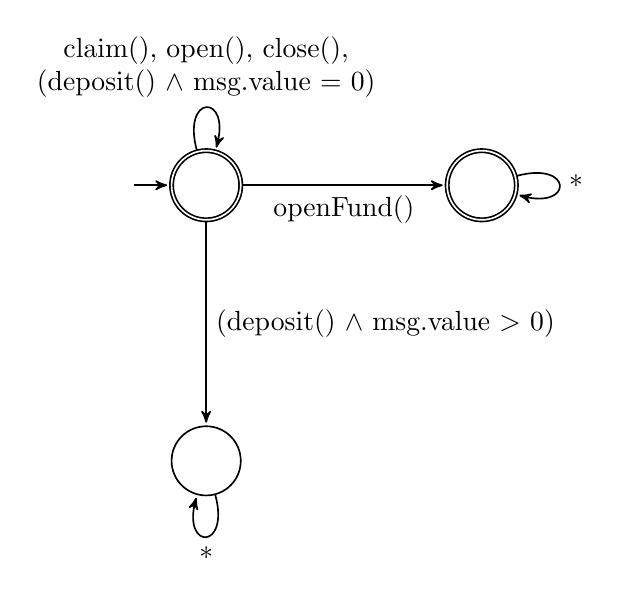
\begin{tikzpicture}[
    ->,
    >=stealth',
    shorten >=1pt,
    auto,
    node distance=3.5cm,
    semithick,
    initial text=$ $
]
	\node[state,accepting,initial] (Init) {};  
	\node[state,accepting] (Good) [right of=Init] {};
	\node[state] (Bad) [below of=Init] {};

	\path[->]
		(Init) edge node {(deposit() $\land$ msg.value $>$ 0)} (Bad)
        (Init) edge [below] node {openFund()} (Good)
        (Bad) edge [loop below] node {*} (Bad)
        (Good) edge [loop right] node {*} (Good)
        (Init) edge [loop above,align=center] node {
            claim(), open(), close(),\\(deposit() $\land$ msg.value $=$ 0)
        } (Init);
\end{tikzpicture}

\end{document}
